%!TEX root = ../thesis.tex

\chapter{引言}

\section{我国债券违约历史}

自 2014 年“11 超日债”违约以来,我国信用债市场中投资者“刚性兑付”的信念逐步动摇、破灭、走向成熟。及至 2021 年,永城煤电、华晨宝马的违约打破了人们对 AAA 级国企的“刚兑信仰”,恒大、海航违约使人们意识到并不存在所谓“大而不倒”,投资者对债券投资逐步恢复理性,我国债券市场也愈发成熟,对债券违约的认识也愈发深刻。一些典型的债券违约事件如表\ref{tab:defaults_in_history}所示。
\begin{table}
	\caption{历史上的重要违约}
	\centering
	\begin{tabular}{lccc}
		债券             & 违约日期   & 原因               & 影响                   \\ \hline
		11 超日债        & 2014-03-05 & 过度扩张资金链断裂 & 打破刚兑的开始         \\
		11天威MTN2       & 2015-04-21 & 经营亏损资不抵债   & 打破国企刚兑           \\
		14波鸿CP001      & 2015-04-12 & “技术性”违约       & 首例“技术性违约”       \\
		15五洋债         & 2018-08-16 & 欺诈发行           & 首例公司债券欺诈发行案 \\
		16民生投资PPN001 & 2019-01-29 & “技术性”违约       & AAA 债券违约第一例     \\
		20永煤SCP003     & 2020-11-26 & 逃废债             & 河南全省融资环境恶化   \\
		15天安人寿       & 2020-12-29 & 股东抽血           & 金融机构破刚兑付       \\
		17幸福基业MTN001 & 2021-02-27 & 过度扩张遇宏观调控 & 地产债违约潮的开始     \\
	\end{tabular}
	\label{tab:defaults_in_history}
\end{table}
套用托尔斯泰的开场白,成功的企业都是相似的,失败的企业却各有各的不同。
我国债券市场的交易额相较于债券市场的体量非常小,违约是小概率事件,成功兑付的债券似乎是天经地义,走向违约的企业各有各的说辞:或称技术原因场外兑付(中融新大),或怨评级公司下调评级(花样年、新力),或称公司流动性遇到了暂时困难(恒大)。债务违约的危害是多层次的:对投资人意味着损失;对发行人意味着丧失外部融资功能、经营难以维系;此外违约还有外部性:如果处理不好可能会影响投融资环境,进而会对整个经济体造成影响。

以史为鉴,可知兴替。本文计划从债券违约影响因素出发,研究我国债券市场违约特征,并通过机器学习的方式佐证、拓展计量模型,以期对债券市场有一个比较好的刻画。

\section{文献综述}
\label{sec:zs}
对于企业违约,不少学者提出过深刻见解。

信用评级是企业违约风险最直观的表述之一,不少学者从信用评级的角度研究企业违约。难以否认的是,我国信用评级市场存在很大的不完善,信用评级比较扭曲,如图\ref{fig:rating}所示,一半为最高评级 AAA 。
这很大程度上是由于发行人付费的模式引起的。\Textcite{吴育辉2020} 指出,“发行人付费”模式下,信用评级虽然可以在一定程度上包含公司的内部私有信息,但由于独立性缺失问题,其总体的信用评级质量仍然低于“投资人付费”模式下的信用 评级质量。此外评级机构竞争为了获得收入也会对公司虚高评级,这是国际评级机构也无法避免的。
评级往往是为了维护发行人利益,初始给予很高的评级,随后在违约事件已经板上钉钉时几天内连续下调原先的虚高评级至垃圾级。\autocite{陈关亭2021多重信用评级与债券融资成本}就对这种现象发出强烈抨击,认为竞争付费导致评级机构存在评级偏差,部分评级机构声誉较差。
事实上,被\autocite{王雄元2013声誉机制}列为低声誉评级机构的大公国际,因涉嫌帮助欺诈发行“五洋债”,应承担 10\% 的连带责任赔偿 7400 万元。但大公竟称“公司已经发不出工资,顶多赔偿150万元”,最终被列入失信被执行人,可见某些评级机构对自身声誉的重视程度。

不仅仅是国内,国外也有学者提出评级可能是最差的信用评估方式\autocite{blochlinger2018ratings},债券交易的价格可能更有效\autocite{badoer2019relevance}。我国也是如此,债券价格大幅偏离估值往往是违约的先兆,一般认为面值100的债券价格下跌至60元左右相当于即将违约,已经违约的债券往往价格只有20元左右。但单纯以价格异动预测违约存在不少假阳性情况,特别是在城投债中,弱省市的城投债成交收益率有时能达到20\%乃至更高。

\begin{figure}
	\centering
	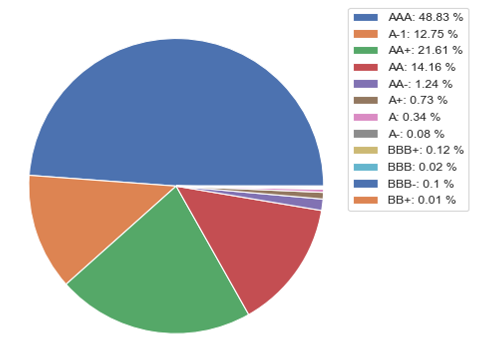
\includegraphics[width=0.9\linewidth]{./data/rating_from_2014.png}
	\caption{\label{fig:rating}信用债发行评级统计}
\end{figure}

公司层面的研究很多还有涉及到公司治理方面的研究。
\Textcite{林晚发2018高管任职经历的得与失}从高管任职经历出发,发现有高管担任过人大代表或政协委员的企业债券发行成功率更高,
\Textcite{anginer2018corporate}提出一个涵盖管理、约束、独立三方面指标的公司治理指标,并指出公司治理增加一个标准差使银行的违约距离指标降低了 0.14 个标准差。
\Textcite{ding2021corporate}和\Textcite{subrahmanyam2017credit}分别从疫情和引入 CDS 对公司治理的影响出发,研究外生冲击由于公司治理能力的差异影响偿债能力的差异。

宏观层面
\Textcite{bai2019common}和\Textcite{bali2021macroeconomic}分别从宏观经济下行和宏观经济不确定性出发,研究宏观环境对于公司债利差的影响。
\Textcite{梅冬州2021财政扩张}和\Textcite{2020Fiscal} 则认为财政扩张导致挤出效应,从而民企面临融资困境,进而违约率上升,利差走阔。
\Textcite{王博2019货币政策不确定性}指出货币政策不确定性的增加会带来违约风险的上升。此外,流动性可能会影响违约\autocite{brogaard2017stock},更高的流动性可以通过提高价格效率来降低违约风险,或者通过放松投资者的退出能力来改善公司治理。

最后还有风险传染角度,有关研究主要集中在系统性风险传染。
\Textcite{苟文均2016债务杠杆与系统性风险传染机制}基于 CCA 模型,提出杠杆率应从较高居民转移至政府等低杠杆部门,以降低违约风险。
\Textcite{2020Do} VAR 模型,认为几乎所有的系统性风险指标对对违约率都有预测能力。
\Textcite{azizpour2018exploring}则认为公司之间的财务、法律或业务关系可能充当风险分散的渠道,通过捕捉系统性风险和这种非系统性的聚类,可以几乎完美地匹配了的时间变化结果所隐含的时间变化的违约计数和违约时间的理论分布。
